%%%%%%%%%%%%%%%%%%%%%%%%
%% Sample use of the infthesis class to prepare a thesis. This can be used as 
%% a template to produce your own thesis.
%%
%% The title, abstract and so on are taken from Martin Reddy's csthesis class
%% documentation.
%%
%% MEF, October 2002
%%%%%%%%%%%%%%%%%%%%%%%%

%%%%
%% Load the class. Put any options that you want here (see the documentation
%% for the list of options). The following are samples for each type of
%% thesis:
%%
%% Note: you can also specify any of the following options:
%%  logo: put a University of Edinburgh logo onto the title page
%%  frontabs: put the abstract onto the title page
%%  deptreport: produce a title page that fits into a Computer Science
%%      departmental cover [not sure if this actually works]
%%  singlespacing, fullspacing, doublespacing: choose line spacing
%%  oneside, twoside: specify a one-sided or two-sided thesis
%%  10pt, 11pt, 12pt: choose a font size
%%  centrechapter, leftchapter, rightchapter: alignment of chapter headings
%%  sansheadings, normalheadings: headings and captions in sans-serif
%%      (default) or in the same font as the rest of the thesis
%%  [no]listsintoc: put list of figures/tables in table of contents (default:
%%      not)
%%  romanprepages, plainprepages: number the preliminary pages with Roman
%%      numerals (default) or consecutively with the rest of the thesis
%%  parskip: don't indent paragraphs, put a blank line between instead
%%  abbrevs: define a list of useful abbreviations (see documentation)
%%  draft: produce a single-spaced, double-sided thesis with narrow margins
%%
%% For a PhD thesis -- you must also specify a research institute:
%\documentclass[phd,cisa,twoside,logo,parskip]{infthesis}

%% For an MPhil thesis -- also needs an institute
% \documentclass[mphil,ianc]{infthesis}

%% MSc by Research, which also needs an institute
% \documentclass[mscres,irr]{infthesis}

%% Taught MSc -- specify a particular degree instead. If none is specified,
%% "MSc in Informatics" is used.
% \documentclass[msc,cogsci]{infthesis}
 \documentclass[msc]{infthesis}  % for the MSc in Informatics

%% Undergraduate project -- specify the degree course and project type
%% separately
% \documentclass[bsc]{infthesis}
% \course{Artificial Intelligence and Psychology}
% \project{Fourth Year Project Report}

%% Put any \usepackage commands you want to use right here; the following is 
%% an example:
\usepackage[numbers]{natbib}
%\usepackage{hyperref}
\usepackage{graphicx}
\usepackage{amssymb}
\usepackage{epstopdf}
\usepackage{parskip}
\usepackage{setspace} 
\usepackage{algorithm}
\usepackage{algpseudocode}
\usepackage{enumitem}
\renewcommand{\rmdefault}{pplx}
%% Information about the title, etc.
\title{Improving the discovery of Motifs in high-dimensional sequences of varying length}
\author{M. Adnan Haider}

%% If the year of submission is not the current year, uncomment this line and 
%% specify it here:
% \submityear{1785}

%% Optionally, specify the graduation month and year:
% \graduationdate{February 1786}

%% Specify the abstract here.
\abstract{%
    %This doctoral thesis will present the results of my work into the
    %reanimation of lifeless human tissues.
}

%% Now we start with the actual document.
\begin{document}

%% First, the preliminary pages
\begin{preliminary}

%% This creates the title page
\maketitle

%% Acknowledgements
\begin{acknowledgements}
Many thanks to my mummy for the numerous packed lunches; and of course to
Igor, my faithful lab assistant.
\end{acknowledgements}

%% Next we need to have the declaration.
\standarddeclaration

%% Finally, a dedication (this is optional -- uncomment the following line if
%% you want one).
% \dedication{To my mummy.}

%% Create the table of contents
\tableofcontents

%% If you want a list of figures or tables, uncomment the appropriate line(s)
% \listoffigures
% \listoftables

\end{preliminary}

%%%%%%%%
%% Include your chapter files here. See the sample chapter file for the basic
%% format.
\include{chapter1}
\chapter{Introduction}

Over the course of the last decade, the mining of time-series data have received considerable attention within the  data mining and machine learning community. The term 'time series' denotes a set of observations concurring any activity against different  periods of time. The duration of time period may be  either in the order of milliseconds or monthly or even annually depending on the domain. 

Mathematically, a time series is defined by the values $y_1, y_2...y_n$ at times  $t_1,t_2... t_n$  where $y=f(t)$.  The time $t_i$  acts as an independent variable to estimate dependent variables $y_i$. The dimensionality of the  series is denoted as \textbf{n} where `\textbf{n}' denotes the length of the sequence. 

 Time series analysis is used in many applications ranging from  sales forecasting, budgetary analysis to stock market analysis and many more. One particular domain where the application of time series analysis is currently very popular is \emph{motif} discovery- the problem of efficiently locating frequent/interesting sub-patterns in the data.  The knowledge of motifs has been seen  to have important applications in various aspects of data mining tasks. For instance motifs can use applied :

 \begin{itemize}
\item  to discover association rules \citep{GautamDas}.  the reflect information of `primitive shapes. 
\item to specify the number of clusters for  unsupervised clustering algorithms. Clustering is one of the most frequently used data mining tasks. It involves an unsupervised process  for partitioning  a dataset into a specified number of  meaningful groups. The knowledge of motifs give a good approximation on the number of meaningful groups that are present in the data. \citep{Fayyad1998}.
\item to identify important sub-patterns in DNA and gene sequences \citep{BRAZMA1998}

\end{itemize}



In the analysis of speech data, motifs  also play a very important role. Recent research have shown that detecting and isolating motifs in speech  utterances is equivalent to extracting frequently spoken words spoken by the speaker(s) \citep{Park2008,Zhang2010}. The methodology proposed in these papers  is based on constructing  a framework that is entirely data driven  i.e there is no intermediate recognition stage  that maps an audio signal to a symbolic representation such as the `phone' states in the HMM model. This  results in   the word acquisition process to be unsupervised which presents a  completely   different approach to the current speech recognition systems that are built using a supervised  training methodology employing  manually transcribed speech to model the underlying speech process.

  
To identify and extract motifs from time series data, various clustering algorithms have been proposed. The two most commonly used approaches are:
\begin{enumerate}
\item Dynamic time warping  algorithm(DTW) \citep{Salvador,Sakoe1990,Rabiner1978,Xie2010,Xi2006,Fu2007} that clusters similar sequences separated by time shifts and/or scale.
\item Single value decomposition(SVD)\citep{Korn1997}. The entire time series data is approximated by a low-rank approximation matrix achieved through mapping the data onto a low dimensional orthogonal feature space.
\end{enumerate}
 Both these algorithms suffer from severe setbacks when applied directly on the `raw' time series data. The DTW algorithm for example, suffers from large run-times when the length of the time series sequences are very long. This is because  the  time complexity of the algorithm  is quadratic and is dependent on the dimensionality of the sequences i.e the length of the sequences.  To address this issue window constraints (Itakura parallelogram\citep{Itakura1975}, Sakoe-Chiba band\citep{Sakoe1990}) are imposed that reduces  size of the search space by forcing the algorithm to look for optimal path that are along the diagonal. Although introducing the window constraint does improve the time complexity  but the reduction the search space leads to a substantial decrease in the accuracy of the algorithm\citep{Fu2007}.

The SVD on the other hand also suffers from high computational cost when the number of samples $\ll$ the size of the dimension of the data. For long time sequences, the high computational cost incurred by the SVD is  therefore quite pronounced as each point in the time series corresponds to a feature/attribute. However, the main drawback of SVD is that it cannot be applied to time-series datasets where the length of the sequences vary. This constraint greatly reduces the type of  time series domains to which SVD  can be applied to. The speech corpus is an  prime example of one such domain where SVD cannot be applied directly. Data sets comprised of  speech utterances are a good example where recorded utterances do not share the same  dimensionality (i.e  the same length) as  acoustically similar signals may be contracted/expanded versions of each other due to speaker variations, context etc.

The purpose of this project is  to employ machine learning techniques to tackle and resolve the drawbacks incurred by both algorithms and thus improve their performance in handling long time series sequences that vary in length. In the  first half of the project, I will be solely concentrating  on improving the performance of the DTW algorithm in problem domains where the minimising the time complexity is a high priority. In the second half of the project, I will investigating ways to  successfully adapt the SVD to work on long sequences that vary in length.



%The discovery of motifs in high dimensional time series data(i.e long sequences) that vary in length  is still a difficult problem to work with. To address the drawbacks of DTW and SVD, there has been some recent work conducted to improve these algorithms. In the paper `` \emph {Fast time series classification using numerosity reduction}", the authors address the drawbacks of DTW in handling high dimensional sequences. They propose an adaptive approach that initially uses a strict window constraint to reduce the search space of DTW but then gradually increase size of the window by discarding samples from the training set. Although this methodology improves the time complexity of the dynamic time warping algorithm by heuristically discarding regions in the input space, the methodology is more tailored to  smart data selection rather than improving the algorithm itself. In the case of SVD, for high dimensional time series sequences which vary in length, the  data matrix  suffers in being  incomplete. Carelessly addressing only the relatively few known entries is highly prone to over �tting. Earlier works [21] relied on imputation to fill  in missing ratings and make the rating matrix dense. However, imputation can be very expensive as it significantly  increases the amount of data. In addition, the data may be considerably distorted due to inaccurate imputation. 
For this project, I will be using 3 time series data sets (details in chapter 2):
\begin{itemize}
\item TIGITS 
\item INLINESKATE
\item CINC\_ECG\_TORSO
\end{itemize}
The prime objective here is to improve the accuracy of the DTW and SVD algorithm in tackling high dimensional time series sequences that vary in length while minimising the run-time to a minimum. To evaluate and compare the merits of different proposed changes, I combined both algorithms with the  K nearest neighbour classifier and  partitioned each of the above data sets into two disjoints subsets: one to be used as  a test set and  the other as a training set.  The reason for choosing the nearest neighbour classifier is because it shares almost the same methodology as the algorithms  used to detect motifs. Motif detection algorithms are memory based i.e they rely on comparing each sequence with other sequences in the data set.  K nearest neighbours deters from motif detection on two aspects: each sequence in the test set is compared with sequences that belong only to the training data set and the entire process is supervised i.e correct label information are available to check the accuracy of the algorithm.  The availability of correct labels allow accuracy and run-time scores of the nearest neighbour methods to serve as a useful evaluation metric to compare and evaluate various adaptions of the DTW and SVD algorithm. Improvements in SVD and DTW that lead to greater classification accuracy scores and low run-times are mostly likely to result in better extraction of motifs in the unsupervised context. 



%For a majority portion of the analysis, the TIDIGITS corpus will serve as  the primary dataset used  to investigate the performances of different models. The reason being the TIGITS corpus consists  of long time series sequences that vary in length . Since each  time sequence corresponds to a speech utterance spoken by a speaker, as result of environment, context and speaker differences the length of the time series sequences will not be the same. In comparison, the sequences with in each UCR data set share the same dimensionality i.e length. Furthermore, the length of the time series sequences on average is much higher in the TIDIGITS corpus than sequences of any data set in the UCR time series database.Thus the TIDIGITS data set is an ideal choice to investigate  the performance of different models in my project.
 %The discovery of motifs in high dimensional time series data that vary in length  is still a difficult problem to work with. Current works have only tried to address the issue of high-dimensional spaces. The state of the art algorithms have been to designed to work on high-dimensional time series sequences that all share the same length. To my knowledge, there exits no algorithm apart from DTW that can applied to high-dimensional sequences varying in length.  Using this as motivation, the aim of this project is to investigate methods  that can improve the discovery of motifs in  high-dimensional time-series sequences that vary in length. In this project, I particularly focus on improving the performance of the DTW algorithm in high dimensional spaces and in the later chapters investigate on  how to adapt unsupervised parametric models to high dimensional  data sets  that vary in length. 

The  dissertation is  organised as follows: Chapter 2 gives a description of the 3 time-series datasets used for this project. Chapter 4  provides a detailed back ground description of the DTW algorithm. Chapter 3 and 4 investigates methods to improve the performance of the DTW algorithm in terms of both accuracy and speed. Chapter4...
\include{chap3}
\chapter{Datasets}
The primary dataset that I have used for this project is the `TIGITS' corpus. (I need to give more description here)

For Training : The entire training data is used
--To contain the computational complexitiy, I am usig samples from production 'a'


For the training set : 
To reduce the average mean time , I am using half of the training data set by choosing samples from one production:
I have chosen:

 225 samples from the boy category
 
 234 samples from the girl category
 
 495 samples from the men category
 
 513 samples from the women category
 

Note : the size of the training set is half of the original training set but contains examples of all classes [1-9]  

For the  test set : Due to the high computational complexity, I  am using only 1/3 of the test set
I have chosen 
162 random samples from boys

162 random samples from girls

326 random samples from men

326 random samples from women

Apart from the TIGITS, I have used two datasets from the UCR database:

The description of the data sets used for the next set of experiments are as follows:
  \begin{enumerate}
  \item CinC\_ECG\_torso
  
  \begin{itemize}
    \item Length of the time series:1639
  \item Size of test set:1380
  \item Size of training set:40
  \item Number of classes:4
  \end{itemize}
  \item  InLineSkate
  \begin{itemize}
    \item Length of the time series:1882
  \item Size of test set:550
  \item Size of training set:100
  \item Number of classes:7 
  \end{itemize}
 \end{enumerate}
  \include{chap2}

\chapter{DTW-Background}
The Dynamic Time Warping algorithm measures the similarity between  sequences varying in both time and speed. Formally, the problem formulation of the algorithm is stated as follows: Given two time series X, and Y, of lengths $|X|$ and $|Y|$,
\begin{eqnarray}
X &= &x_1,x_2...x_{|X|}\\
Y &= &y_1,y_2...y_{|Y|}
\end{eqnarray}
construct a warping path W
\[ W =  w_1, w_2...w_k \mbox{ where max } (|X|,|Y|\leq k\leq |X|=|Y|\]
\begin{itemize}
\item Here \emph{k} denotes the length of the warping path and the  mth element of the warping path is $w_l = (n_l,m_l) \in [1 : N]\times[1 : M] \mbox{for } l \in [1 : k]$ where $n_l$ is an index from the  time series X and $m_l$ is an index from the time series Y.
\end{itemize}
To  properly understand  the  mechanism of the DTW algorithm, the definition of some key terminologies  must first be stated:
 \begin {enumerate}
\item Warping path:
An (N,M)-warping path (or simply referred to as warping path if N and M are clear from the context) is a sequence $w= (w_1,...,w_k)$ with $w_l = (n_l,m_l) \in [1 : N]\times[1 : M] \mbox{for } l \in [1 : k]$ satisfying the following three conditions.
 \begin{enumerate}
 \item Boundary condition: $p_1 = (1,1)$ and $p_k = (N,M)$.
 The boundary condition enforces that the first elements of X and Y as well as the last elements of X and Y to be  aligned with each other. In other words, the alignment refers to the entire sequences X and Y.
 \item Monotonicity condition requires that  the path will not turn back on itself, both the i and j indexes either stay the same or increase, they never decrease. 
 
 \item Step-size condition: $p_{l+1}-p_l \in \{(1,0),(0,1),(1,1)\}$  for l $\in$ [1:k-1].
 The step size con- dition expresses a kind of continuity condition: no element in X and Y can be omitted and there are no replications in the alignment
 \end {enumerate}
 Intuitively speaking, the (N,M)warping path$ p = (p_1,...,p_k) $defines an alignment  between two sequences $X = (x_1,x_2,...,x_N)$ and $Y = (y)1,y_2,...,y_M)$ by assigning the element $x_i$ of X to the element $y_j$	of Y.   
 \item Optimum Warping Path :
 
 The optimal warp path corresponds to the  minimum-distance warp path, where the distance of a warp path W is given as 
 \[ Dist(W) = \sum_{i=1}^{K} dist(X,Y)_{|(w_i)}\]
 $dist(X,Y)_{|(w_i)}$  represents the distance computed using an appropriate  cost function between the time series points of $x_{ni}$ of sequence X and $y_{mi}$ of sequence Y. \[\emph dist(X,Y)_{|(w_i)} = dist(x_{ni},y_{mi}) \]
 
\end{enumerate}
The goal of the DTW algorithm is to compute the distance of the optimal warping path between two time series sequences. Instead of attempting to solve the entire problem all at once, the  algorithm utilises the technique of dynamic programming to find an optimum alignment between two sequences through the computation of local distances between the points in the temporal sequences. The algorithm proceeds by  iteratively filling in values for each cell (i,j) in  the  $|X|$ by $|Y|$ cost matrix \emph{D}. The value of the cell (i,j) is given by  $D(x_{ni}, y_{mj})$  which corresponds to the minimum- distance warp path :
\[D(i,j) =Dist(i,j) +min(D(i-1,j),D(i-1,j-1),D(i,j-1))\]
An outline of the baseline DTW algorithm is given below:

 \begin{algorithm}[H]

\begin{algorithmic}[1]
\Procedure{Value-based}{$seq1,seq2$}\Comment{two raw sequences }
\State DTW= zeros(length(seq1)+1,length(seq2)+1)
 \For{i=1: to length(seq1) }\Comment{Initialise the DTW cost matrix}
 \State DTW(i,0) = $\infty$
 \EndFor
 
 \For{i=1 to length(seq2)}
 \State DTW(0,i) = $\infty$
 \EndFor
 
  \For{i=2 to length(seq1)}  
 \For{j=2 to length(seq2)} \Comment { cost(a,b)$\equiv$euclid(a,b)}
 \State DTW(i,j) = cost(seq1(i),seq2(j)) + min\{ DTW(i-1,j)+DTW(i,j-1)+DTW(i-1,j-1)\}
 \EndFor
 
 \EndFor
\State \textbf{return}  result = $\frac{\mbox{DTW(n,m)}}{nm}$ \Comment{n=length(seq1), m=length(seq2)}

\EndProcedure 
\end{algorithmic}
\caption{Value-Based DTW}
\end{algorithm}
The figure below gives an example of the optimal path found by the algorithm.
\begin{figure}[H]
  \centering
   
     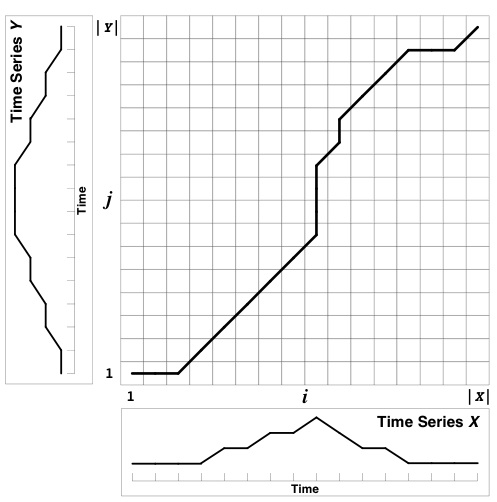
\includegraphics[scale=0.8]{DTWpicture.jpg}
  \caption{A cost matrix with the minimum-distance warp path traced through it.  }
  \end{figure}
  The computational complexity of the DTW algorithm is \emph{O}($n^2$) where $n$ denotes the length of the sequences that are being compared. Thus for time series domains having high dimensions(long sequences), the time and computational costs incurred by the algorithm are quite high.  To address this issue, two well-known global window constraints are employed:  the Sakoe-Chiba band[18] and
the Itakura parallelogram[19] . Figure 3.2  gives an illustration of the use of both constraints:
  \begin{figure}[H]
  \centering
   
     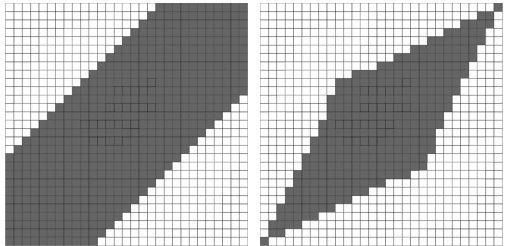
\includegraphics[scale=0.8]{windowconstraint.jpg}
     \caption{ Two constraints: Sakoe-Chuba Band (left) and an Itakura Parallelogram (right), both have a width of 5.}
    \end{figure}
  
 The Sakoe-Chiba band runs along the main diagonal and has a fixed (horizontal and vertical) width .The Itakura parallelogram  on the other hand describes a region that constrains the slope of a warping path. To constraint the time complexity to a minimum, the vast majority of the data mining researchers use a Sakoe-Chiba Band with a 10\% width.
 
 \include{chap3}
\chapter{Improving DTW}
The Dynamic Time Warping(DTW) algorithm is the one of the oldest algorithms that is used to compare and cluster sequences varying in time, length and speed. Given two temporal sequences, the algorithm utilises the technique of dynamic programming to compute the cost of the optimum alignment path between them.  The computed cost gives an indication of the degree of similarity. The smaller the cost, the more similar the sequences are.Intuitively speaking, DTW is a clustering algorithm that clusters similar patterns varying in time and speed. The time and computational complexity of this algorithm is  \emph{O}($n^2$) where $n$ denotes the length of the sequences that are being compared. Thus for time series domains having high dimensions(long sequences), the time and computational costs incurred by the algorithm are quite high which  makes DTW a very unattractive choice for clustering or discovering motifs in high dimensional  data sets.  Another drawback for working in high-dimensional spaces is the contrast between the distances of nearest and furthest points. The distances between such points  become increasingly smaller  as the dimensionality increases. This makes it  difficult to construct meaningful cluster groups in such spaces.

To address the issue of the curse of dimensionality, DTW algorithms employ a window constraint to reduce the search space. The most commonly used  are Sakoe-Chuba Band[18]  and the Itakura  window constraint[19]. Figure[3.2]  gives an illustration on the nature of these window constraints. These constraints determine the allowable  shapes that a warping path can take by restricting the DTW to find an optimal warping path only through the constrained window. As the dimensionality(length) of the sequences increases, the size of the window is adjusted accordingly. Rigid  window constraints impose a more rigid alignment  that prevent an overly temporal skew between two sequences, by keeping frames of one sequence  from getting too far from the other. The vast majority of the data mining researchers use a Sakoe-Chiba Band with a 10\% width for the global constraint[23] to constraint the time complexity of DTW to a minimum. For clustering data sets such as speech utterances, the effect produced by such global constraints is highly undesirable. If we consider two utterances of a word spoken at different time frames, the patterns can have an overly temporal askew between them as result of the different contexts in which the  words are spoken and/or as a result of  different speakers speaking the same word. Thus it is necessary to explore alternative techniques to window constraints that can reduce the time complexity of  the DTW algorithm to a minimum without decreasing accuracy. 

Before investigating methods to improve the DTW algorithm itself, it is highly necessary to first understand the nature of the data sequences that the DTW is presented with.  By achieving a thorough understanding of the data, we can  achieve dimensionality reduction by  isolating and identifying smaller set of new(current)  features  that are more relevant for the problem in hand.  In this chapter, I investigate domain-dependent preprocessing techniques that can improve  the  DTW's performance by mapping   the sequences  to a lower dimensional space that captures the intrinsic structure of the data.
 There are presently two groups of preprocessing techniques commonly used to address this issue:
\begin{itemize}
\item  Feature Selection 
\item Feature Extraction
\end{itemize}
 Feature selection techniques  involve selecting only a subset of attributes from the original data. With respect to the time series data, the process refers to sub-sampling the sequence.  One of the most popular approaches to feature selection is  the exploratory data analysis(EDA). EDA is an approach to data analysis that postpones the usual assumptions about what kind of model the data follows with the more direct approach of allowing the data itself to reveal its underlying structure and models. The particular techniques employed in EDA are often quite simple, consisting of various techniques of:
 
 \begin{enumerate}
\item Plotting the raw data such as data traces, histograms, histograms, probability plots, lag plots, block plots, and Youden plots.
\item Plotting simple statistics such as mean plots, standard deviation plots, box plots, and main effects plots of the raw data.
\item Positioning such plots so as to maximise our natural pattern-recognition abilities, such as using multiple plots per page.
 \end{enumerate}
Feature extraction processes on the other hand are concerned with  the range of techniques  that apply an appropriate functional mapping to the original attributes to extract new features. The intuition behind feature extraction is that the data vectors $\{x_n\}$ typically lie close to a non- linear manifold whose intrinsic dimensionality is smaller than that of the input space as a result of strong correlations between the input features. Hence by using appropriate functional mapping, we obtain a smaller set of features that capture the intrinsic correlation between the input features. By doing so, we move from working in high dimensional spaces to working in low dimensional spaces. The choice  of appropriate functional mapping can  also improve the clustering of data. For example, lets consider figure 4.1: The left- hand plot represents the locations of two dimensional  data points  in the original input space. The colours red and blue denote the classes to which the data points belong to. To cluster the data with respect to their classes, it will be ideal if we can partition the input space into disjoint regions where points belonging to the same class occupy the same region. This is achieved by mapping the points to a feature space spanned by  two gaussian basis functions(shown on the right). Now, we can partition the feature space into two disjoint regions,, one of each cluster. 




\begin{figure}[H]
  \centering
   
     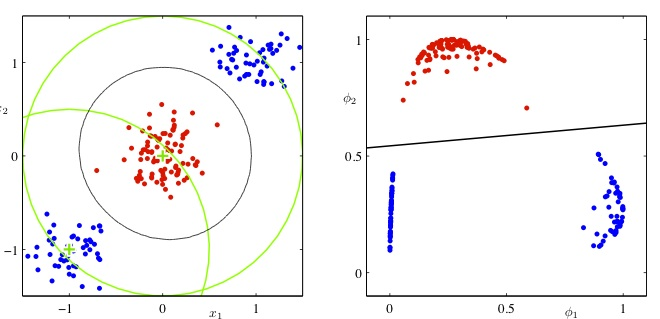
\includegraphics[scale=0.8]{featuremapping.jpg}
  \caption{The figure on the right corresponds to location of the data points in the feature space spanned by gaussian basis functions $\phi_1(x)$ and $\phi_2(x)$ }
  
\end{figure}
In the rest of this chapter,  I explore a range of  feature selection and extraction methods  and investigate whether their application can improve the performance of the DTW algorithm in terms of both accuracy and time complexity.
%The DTW algorithm combined  with the  1 nearest neighbour classifier  is a memory based algorithm. Memory-based methods involve storing the entire training set in order to make predictions for future data points. They typically require a metric to be defined that measures the similarity of any two vectors in input space, and are generally fast to �train� but slow at making predictions for test data points. The time and computational complexity associated with such methods is even higher when the dimensionality of the data points is high. Intuitively speaking, DTW is a clustering algorithm that clusters similar patterns varying in time and speed. In high- dimensional spaces, however, the contrast between the nearest and furthest points gets increasingly smaller, making it difficult to construct meaningful cluster groups. To address this issue, data dimensionality methods are used at the  preprocessing stage.
 
\section{Feature Selection}
The computational and time complexity associated with the DTW algorithm is governed by the dimensionality of the time  series. To get a feel of the data, I employed exploratory data analysis on the  isolated word utterances belonging to the test and training data sets  that I constructed from the TIDIGITS corpus. The aim here   to identify and isolate redundant features from the time series data.
 To get an idea about the structure of the data, I have studied the plots of the time series sequences along with listening to the individual samples. Figure 4.2 gives the plot of raw signal corresponding to the word `8' by a speaker from the \emph{boy} category. From the visual and auditory analysis, I have made the following  observations:
\begin{itemize}
\item Long durations of silence occupy the beginning and end of each utterance.   These durations of silence segments are considerably long compared to the interesting regions in the acoustic signal that actually contain information about the spoken digit .  Removing these silence segments do not only  reduce the dimensionality of the time series but also result in minimal loss of information.
\item  Through listening to  numerous samples, I have discovered that  the recordings are highly distorted when played in \emph{matlab} even when the data is scaled so that the sound is played as loud as possible without clipping. The distorted signal fails to provide any type of auditory clue about  category of the speaker i.e whether the speaker belongs to \{ boy,girl, men,women\}  and the signal must be played multiple times  for the word to be correctly identified.
\end{itemize}
\begin{figure}[H]
  \centering
   
     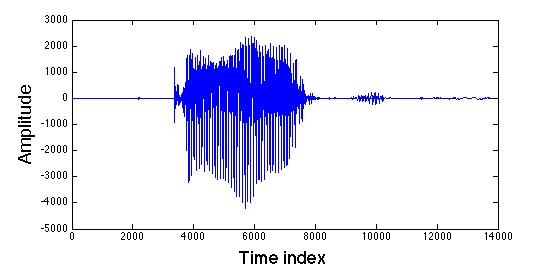
\includegraphics[scale=0.6]{Rawsample.jpg}
  \caption{`Raw 'signal}
  
\end{figure}
\subsection{Signal Filter}
Thus to remove these redundant attributes from the time series sequence, I have constructed  the following algorithm: `silencefilter' that performs feature selection by removing segments of silence.  An outline of the algorithm is as follows:

\begin{algorithm}[h]

\begin{algorithmic}[1]
\Procedure{Silencefilter}{$signal$}\Comment{raw signal }
\State $threshold=0$
\State maxAmplitude= max(rawSignal)
 \State Adapt the threshold based on the value taken by the maximum amplitude
 \State output$\leftarrow$ removeSilence(rawSignal,threshold)
 \State \textbf{return} output%$\leftarrow$ downsample s\_R by $\frac{1}{2}$
 
 \EndProcedure
\end{algorithmic}
 \caption{SignalFilter}
\end{algorithm} 
  The algorithm removes all samples in the times series sequence whose magnitude is less than the threshold. The threshold used is an adaptive parameter. By using the information of the signal's maximum amplitude the algorithm sets the threshold accordingly. It raises the threshold for signals corresponding to speakers having a loud and deep voice   and lowers the threshold for signals corresponding to speakers having gentle and low voice.
  
  
  
 \begin{figure}[H]
  \centering
   
     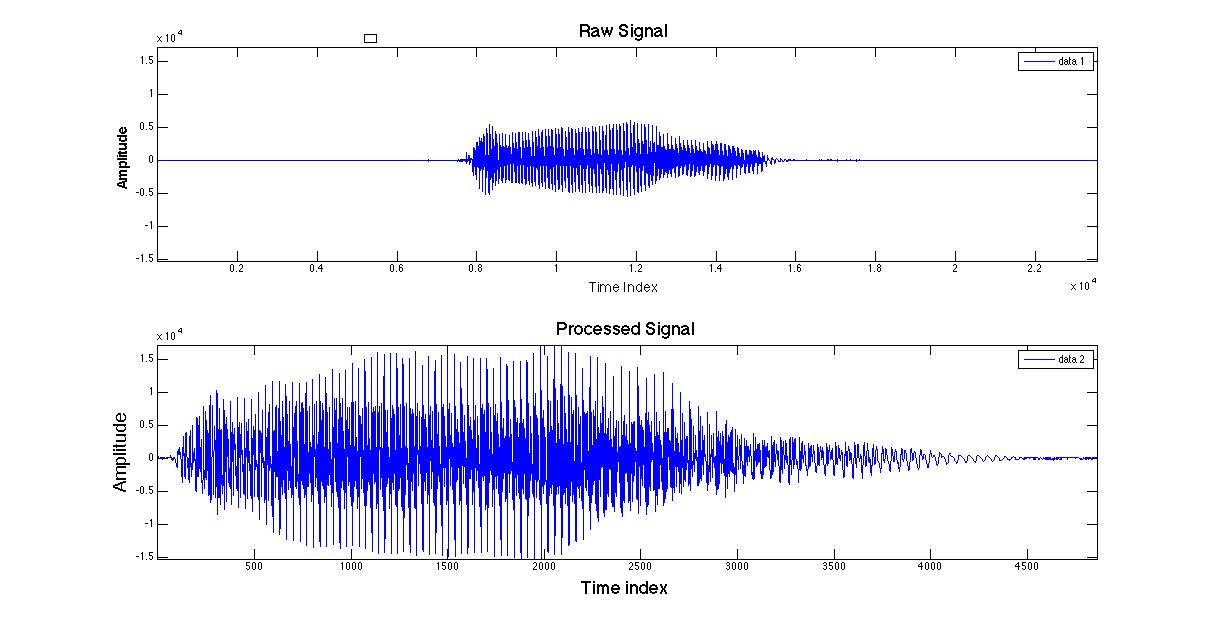
\includegraphics[scale=0.5]{Feature_selection.jpg}
  \caption{shows the raw acoustic signal corresponding to the utterances of the digit '8' alongside with the version that has its dimensionality reduced by the filter discussed above.    }
  \end{figure}
 From figure 4.3, it can be observed that the filter preserves the interesting patterns associated with the utterance while succeeding in reducing the dimensionality of the data. To investigate the effect of  introducing this prior feature selection step  on the  performance of the DTW algorithm , I conducted the following experiment:
 
 \begin{itemize}
 \item Objective : Performance  comparison between  DTW equipped with a feature selection step against the based line DTW
 \item Dataset used: TIDIGITS
 Test-set size : 976 samples

\begin{center} 
 \begin{tabular}{lclcl}
 \hline 
 category &  sample size \\
 boy & 162 \\
 girl & 162\\
 men & 326 \\
 women & 326 \\
 \hline
 \end{tabular}
  \end{center}
  Training  data set size: 1467
  
 \begin{center}
 \begin{tabular}{lclcl}
 \hline 
 category &  sample size \\
 boy & 225 \\
 girl & 234\\
 men & 495 \\
 women & 513 \\
  \end{tabular}
  \end{center}
  \item
  An outline of DTW  used algorithm used for this experiment  is given below.  
 \begin{algorithm}[H]

\begin{algorithmic}[1]
\Procedure{Value-based}{$seq1,seq2$}\Comment{two raw sequences }
\State DTW= zeros(length(seq1)+1,length(seq2)+1)
 \State w = max($\lceil{0.1*max(n.m)}\rceil$, abs(n-m)) \Comment{Window constraint }
 \For{i=1: to length(seq1) }\Comment{Initialise the DTW cost matrix}
 \State DTW(i,0) = $\infty$
 \EndFor
 
 \For{i=1 to length(seq2)}
 \State DTW(0,i) = $\infty$
 \EndFor
 
  \For{i=2 to length(seq1)}  
 \For{j=max(2, i-w) to min(length(seq2), i+w)} \Comment { cost(a,b)$\equiv$euclid(a,b)}
 \State DTW(i,j) = cost(seq1(i),seq2(j)) + min\{ DTW(i-1,j)+DTW(i,j-1)+DTW(i-1,j-1)\}
 \EndFor
 
 \EndFor
\State \textbf{return}  result = $\frac{\mbox{DTW(n,m)}}{nm}$ \Comment{n=length(seq1), m=length(seq2)}

\EndProcedure 
\end{algorithmic}
\caption{Value-Based DTW}
\end{algorithm}
Note : The DTW algorithm is subjected to an adaptive window constraint. The focus of my research here is to improve the accuracy of the DTW algorithm while reducing the time and computational cost to a \textbf{ minimum}. Even after applying the feature selection process, from initial experiments I have found the dimensionality of the time series sequences is still very high. Thus for these experiments, I have employed the Sakoe-Chuba band that is adaptive in  size : w = max($\lceil{0.1*max(n.m)}\rceil$, abs(n-m)). The lower bound of the window size is set to10\%  the size of the longest sequence because its is the standard size that  the  vast majority of the data mining researchers[23] use  to keep the time complexity of DTW to a minimum.
\item RESULTS:

 \begin{figure}[H]
   \centering
   
     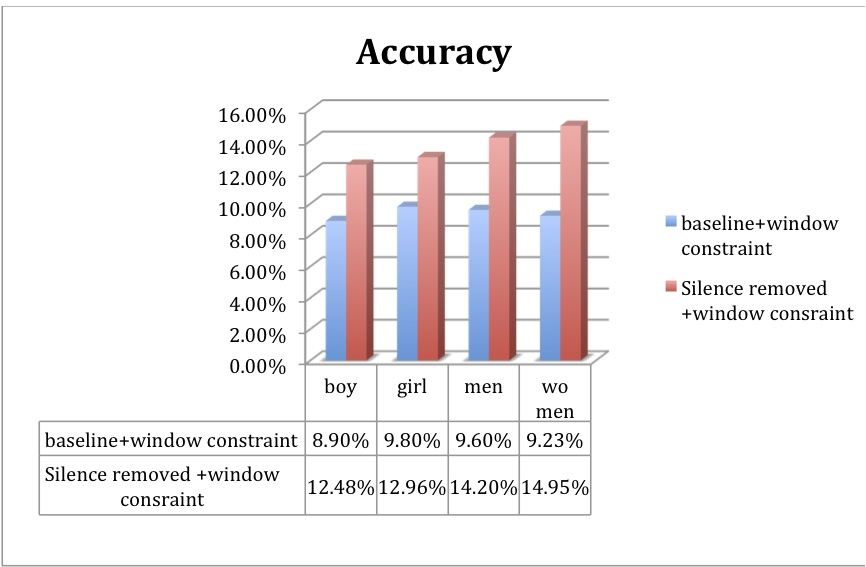
\includegraphics[scale=0.8]{4111.jpg}
  \caption{ }
  
\end{figure}
\begin{figure}[H]
  \centering
   
     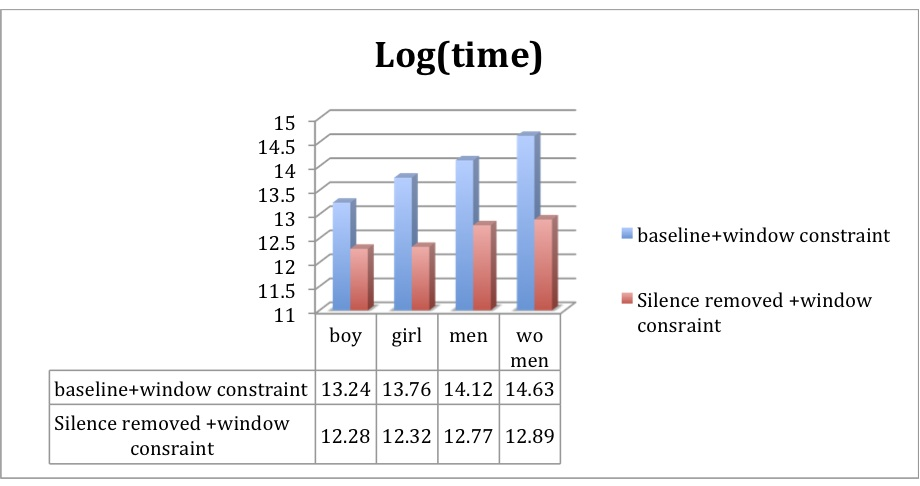
\includegraphics[scale=0.6]{4112.jpg}
  \caption{}
  
\end{figure}
\end{itemize}
Observations:
\begin{itemize}

\item From the results above, it can seen that the  DTW algorithm achieves very poor accuracy. The reason for this lack of poor recall may be attributed to one  or  a combination of the following three factors:
\begin{itemize}
\renewcommand{\labelitemi}{$\rightarrow$}
\item raw values- the value of a data point in a time series sequence is not a complete picture of the data point in relation to the rest of the sequence.
\item window constraint- the optimum warping path exists outside the boundaries of the Sakoe-Chuba bands[3,6].
\item not using MFCC values- The data set comprises of speech utterances. It is a widely known fact that for speech data, the MFCC feature vectors capture the information of phones that make up a word. Since different lexical identities are composed of different phones, these use of these vectors can provide effective clustering. (details of MFCC to follow)[3,4,5,6,7].
 \end{itemize}

 \item Removing `silence' segments improves \textbf{both} the accuracy and the time complexity of the algorithm.
Reasons:

 The DTW algorithm, aims to finds an optimum warping path  in the search space bounded by the window constraints. Removing `silence' segments proves to be highly advantageous because  these `silence' are present in all utterances. Thus there are not good  discriminators for identifying different lexical identities.  Taking these silences into account therefore degrades the performance of the DTW as  they bring in an unwanted notion of similarity in dissimilar patterns.
 
 
 The size of the DTW cost matrix is \emph{O}(mn). Achieving dimensionality reduction through feature selection reduces the size of the cost matrix and thus decreases the computational cost.




\end {itemize}

\subsection{Downsampling}
From further exploratory data analysis,  I have observed that if  I down-sample the utterances by $\frac{1}{2}$  which in other words means decreasing the sampling frequency by half, the resultant sampled signal is much clearer to understand.  From the observation of figure 4.6, it can be seen that performing sub-sampling does keep the global trend of the signal intact but results in minute loss of local information. Furthermore through listening the sampled signals, I have discovered that losing some \textbf{local information} actually cleans the signal in a manner that allows the listener to identify the speaker's category and the lexical identity with ease.
 \begin{figure}[H]
  \centering
   
     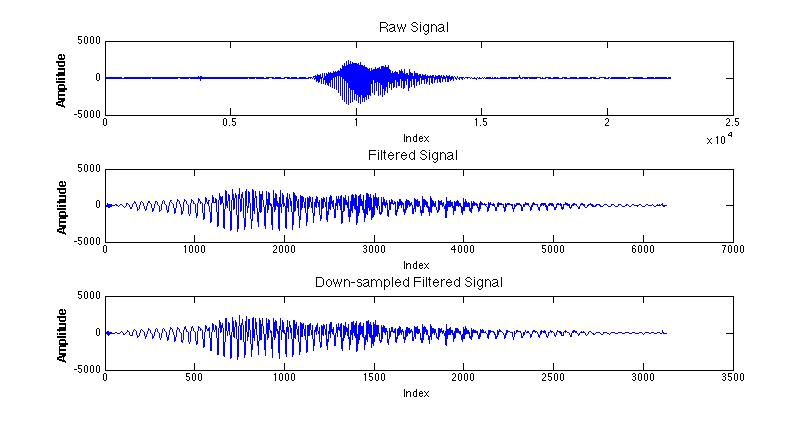
\includegraphics[scale=0.5]{Feature_selection2.jpg}
  \caption{shows the raw acoustic signal of the digit `8' (top figure), the silence removed version of the signal(middle) and the silence removed and down sampled version of the acoustic signal (bottom) }
  \end{figure}
To investigate whether performing further dimensionality reduction  through downsampling improves the performance of the DTW, I conducted a third experiment using the same data set and the sample DTW algorithm discussed in 4.1.1.  The results found are as follows:
 \begin{figure}[H]
   \centering
   
     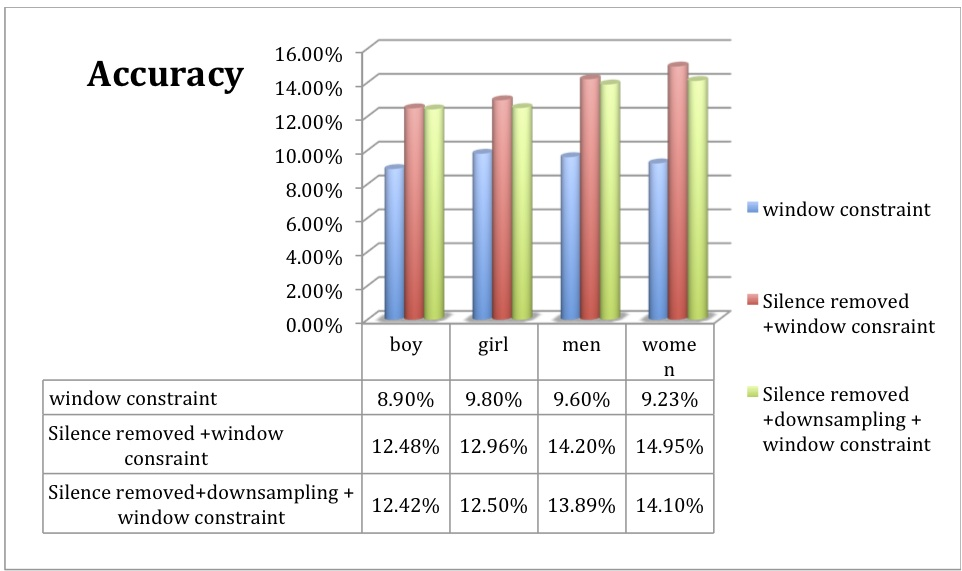
\includegraphics[scale=0.7]{4121.jpg}
  \caption{Performing silence removal followed by downsampling still achieves better accuracy than the base line DTW }
  \end{figure}
 \begin{figure}[H]
   \centering
   
     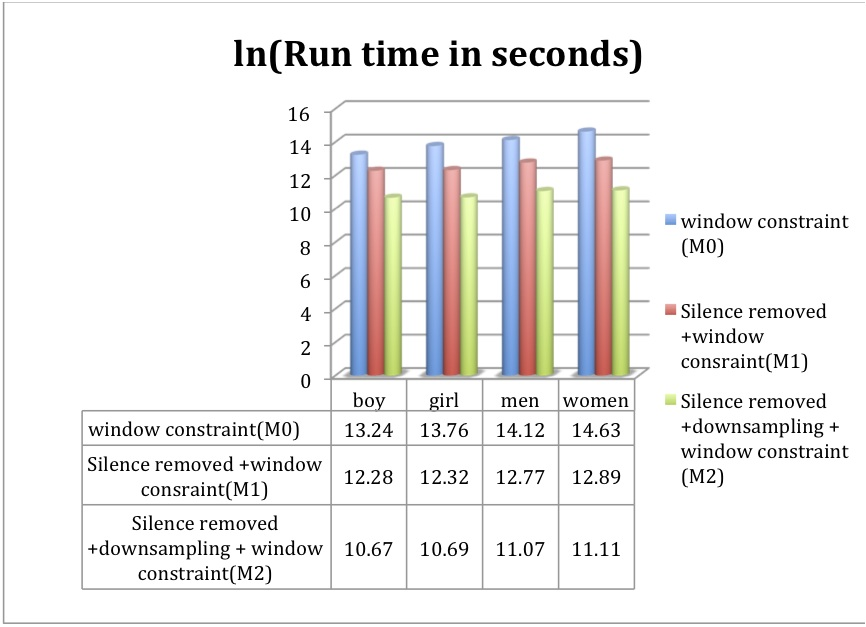
\includegraphics[scale=0.5]{4122.jpg}
     
  \caption{ Integrating downsampling into the preprocessing step decreases the log(time)}
Observations:

\begin{itemize}
\item Performing down-sampling along with silence removal achieve a reduction in the log(time) by 1.5 on average. This is expected since in the first stage of the preprocessing phase, redundant features are dropped which reduces the dimensionality(i.e length ) of the sequences. The length of the sequences is reduced even further through downsampling the the output sequences of stage 1. the computational cost of DTW is directly dependent on the length of the sequences,  thus decrements in dimensionality leads to a decrease in the computational cost.
\item Although  the downsampling method seems to improve the quality of the signal from a listeners viewpoint, the accuracy of the DTW on the down-sampled sequences  is seen to be actually less than the DTW algorithm that employs silence removal as the only pre-processing step.  I found the cause of the anomaly to be `soundsc' function of matlab. The function scales the acoustic signal as loud as possible without clipping causing the resultant signal hard to understand.  The reason for the decrement in accuracy is quite obvious : removing attributes leads to a loss of information.  The DTW's accuracy is reduced by   1\% on average in comparison to the model that uses only silence removal as a pre-processing step. Even through loss
achieves  an accuracy that is 3\% greater on average across the test data sets of all categories  in comparison to the baseline DTW.
\end{itemize}  

\end{figure}

\section{Feature extraction}
From the analysis conducted so far, it can be concluded that heuristically selecting only significant  attributes from the time series sequences does \textbf{improve} the accuracy and the speed of the DTW. However, from the observation of the experimental results,it is quite clear that  the accuracy of the algorithm is very low.  In this section, I investigate on the degree of influence that employing domain-dependent and domain dependent feature extraction methodologies have on the speed and accuracy of the DTW algorithm. There are two motivations behind conducting this analysis:
\begin{itemize}
\item The primary motivation is to investigate  to what degree is this low error credited to not using features that incorporate information about the domain and the trends of the sequence and the degree of  contribution that  using a rigid window constraint has on the low accuracy . (The features that we have considered so far are the raw  values indexed by time)
\item The overall focus is to improve the speed  of the DTW algorithm without degrading accuracy. By choosing an appropriate functional mapping, we can map the data to lower dimensional feature space that can captures the intrinsic qualities of the data. This not achieves dimensionality reduction of the time series sequences but also posses  the potential to boost accuracy.
\end{itemize}

\subsection{Domain-dependent feature extraction}

The primary data set that I am working with for this project  is the TIGITS corpus which is composed of speech utterances. For speech, the most commonly used features are the MFCC features-mel cepstrum ceptral coefficients. This feature representation is based on the idea of the cepstrum. For human speech, a speech waveform is created when a glottal source waveform of a particular frequency is passed through the vocal tract which because of its shape has a particular  filtering characteristic. The exact position of the vocal tract is in fact the key attribute in providing useful information about phones(units of sounds). Cepstrum provides a useful way to separate the information of the vocal tract from the glottal source.

A sketch of the MFCC feature extraction is given below:
\begin{figure}[H]
  \centering
   
     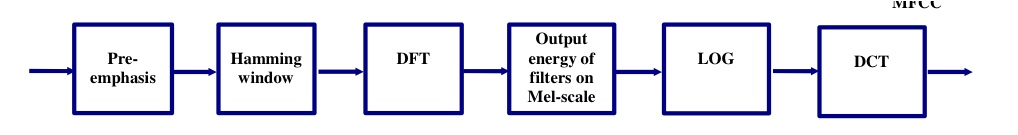
\includegraphics[scale=0.8]{mfcc.jpg}
  \caption{MFCC feature extraction}
  \end{figure}
\begin{enumerate}[label=\roman*]
\item Pre-emphasis: boosts the energy of the signal at high frequencies to improve phone detection
\item Windowing: partitions the time series sequence into frames using a hamming window
\item DFT: extracts spectral information at different frequency bands
\item Mel scale : transforming to mel scale improves recognition performance by allowing the model to take into account the property of human hearing
\item Log : makes the feature less sensitive to variations in input such as power variations on the speakers mouth.
\item Cepstrum : separate the information of the vocal tract from the glottal source. The first 12 cepstral values from spectrum of the log of the spectrum  are used
\end{enumerate}

Through the windowing process, the MFCC features extraction achieves dimensionality reduction. Each sequence is segmented into frames of length 20 to 30 ms which are then through appropriate functional mapping  are converted into sequences of MFCC feature vectors. Since the result sequence of vectors is much smaller than the length of the original sequence resulting in the size of the DTW cost matrix is much smaller than before, This in turn lowers the time and computation cost incurred by the algorithm.

The experiments conducted in section 4.1.1 and 4.1.2, have shown that the  DTW algorithm performs very poorly in terms of accuracy on the TIDIGITS test data when it employed a very constrained window to reduce the time complexity to a minimum. The reason for this low accuracy was narrowed down to one or  a combination of these factors : using a narrow window constraint, raw attribute values and not incorporating the use of domain and structural properties of the signal in the features(attributes). To investigate the influence of  each these  individual factors on the performance of DTW, I constructed the following 3 models:
\begin{enumerate}[label=\roman{*}]
\item Model 1  employs MFCC feature extraction as a preprocessing step and then runs the DTW algorithm  using the same window constraint  mentioned in 4.1.1. The  performance of this model can be used to investigate the contribution of using domain-dependent features in the performance of the DTW algorithm. 
\item  Model 2 employs a two stage preprocessing step. The feature selection procedure  discussed in 4.1.1  is first applied to remove redundant features followed by MFCC feature extraction that achieves further dimensionality reduction(i.e reduction in length of the sequences) . In this model dimensionality reduction occurs at both stages of the pre-processing step.  For these experiments, the downsampling method discussed in 4.1.2  was deemed not necessary  because the feature extraction phase allows greater reduction in dimensionality without any loss of information. The sequence of vectors was then fed to the DTW  algorithm augmented with the window constraint discussed in section 4.1.1.. The performance of this version of  DTW  can be compared with the version 1 DTW to decide on the  pre-processing techniques that yields the best performance.
\item  Model 3  is identical to the version 2  with the exception that this version does not employ the window constraint.   The performance of this version of the DTW  can be compared with the results found in section 4.1.1 and the performance of the other versions to  investigate the influence of using window constraint on the accuracy of the DTW. 

\end{enumerate}
Experimental setup:

  \textbf{Data- set} : The TIDIGITS  training and test set (Chapter 2, 4.1.1)
  
\textbf{RESULTS}:



\begin{figure}[H]
  \centering
   
     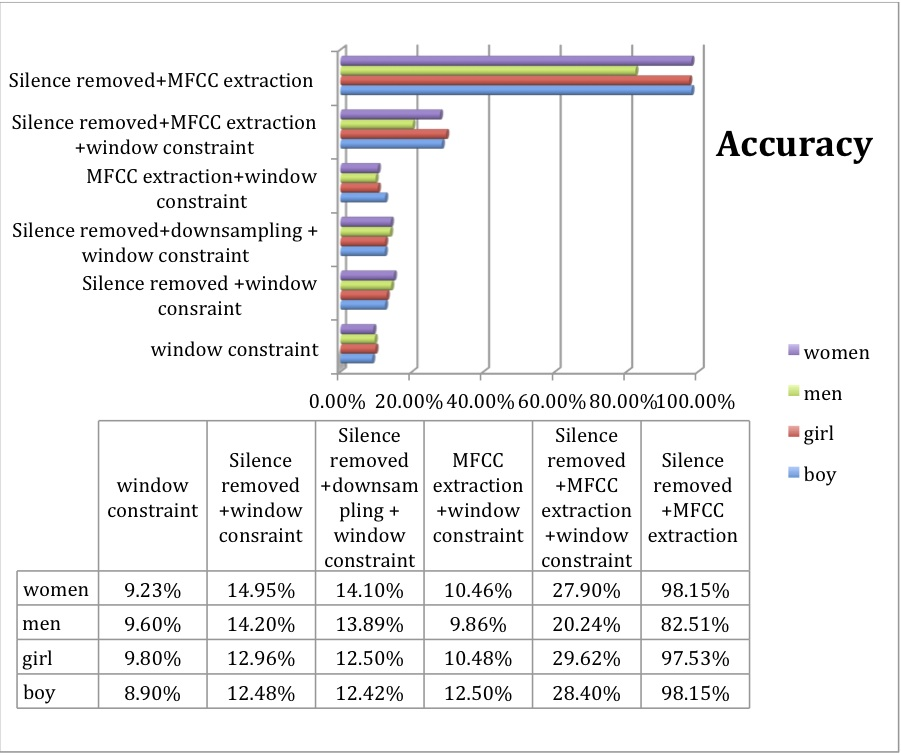
\includegraphics[scale=0.9]{421.jpg}
  \caption{MFCC feature extraction}
  \end{figure}
  
\begin{figure}[H]
  \centering
   
     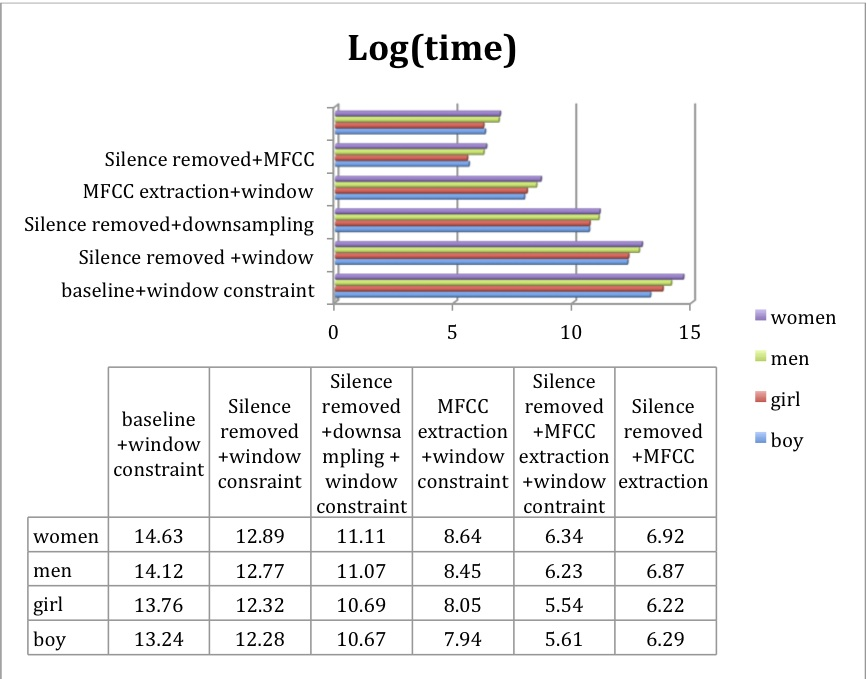
\includegraphics[scale=0.8]{422.jpg}
  \caption{MFCC feature extraction}
  \end{figure}

  Observations:
 
  
  \begin{itemize}


  \item Replacing raw values with MFCC features surprisingly only leads to a minimal increase in the accuracy of the DTW subjected to a window constraint. By comparing these results with the  experiments done in 4.1.1, it can observed that the presence of `silence' forces the optimal warping path between utterances corresponding to identical lexical identities  to occupy regions that are outside those that are bounded by the adaptive Sakoe-Chuba band constraints.
  
   \item Combining  attribute/feature selection with MFCC feature extraction as a preprocessing step achieves greater improvement in accuracy and speed than using either of these approaches alone. In comparison to just using MFCC feature extraction as a preprocessing step, the algorithm's accuracy has been boosted up by 15.17\% on average  while the $log(time)$ have been reduced by 2.36.  Similarly in comparison  to just using feature selection as a preprocessing step, the algorithm's accuracy has  increased  by 12.9\% on average  while the $log(time)$ have been reduced by 6.5.
   
    From this observation alone, we deduce two facts, one of which is not that obvious: the accuracy of the DTW is governed by the removal `silence' segments and the size of the Sakoe-Chuba band constraint.  Since the main focus is to improve  \textbf{both} the accuracy and  speed of DTW in handling sequences of high-dimensionality i.e long lengths, removal of silence segments provides an ideal mechanism to improve the time complexity and the accuracy of the algorithm.
  
  \item Model 3 achieves almost near perfect accuracy. Dropping the window constraint improves the accuracy by 67.15\% on average over model 2.  Thus 67.15\% times on avergage, the optimum warping path lay outside the regions bounded by the Sakoe-Chuba band constraints, This proves  that  patterns belonging to the same lexical identity can have an overly temporal askew between them as result of the different contexts in which the words are spoken and/or as a result of different speakers speaking the same word.
  
  Although removing the window constraint does degrade the time complexity in comparison to the log(time) cost of model 2, if  we compare the log(time) of model 3  with the other models, we can observe that model 3 achieves lower  $log(time)$ s  than any of the model with the exception of model 2.
  

 Therefore from this analysis, it can be concluded that  equipping DTW with  preprocessing techniques constructed by performing exploratory data analysis and  integrating  metadata(i.e knowledge of the domain) can serve as an alternative to equipping the algorithm with rigid window constraints to handle high dimensional time series sequences in terms of both accuracy and speed. 
  % \item It can be observed that adapting DTW to incorporate a pre-processing stage that involves removal of redundant features through silence removal and employing a feature extraction mapping that integrates domains knowledge in the feature extraction process achieves almost perfects accuracy and incurs the lowest computational time. To be precise, adapting DTW to be domain-dependent allows the algorithm to achieve near perfect accuracy while incurring the minimum computational cost. 
  %\item From analysing the time complexity associated with each of the two versions, it can be seen that partitioning the sequences into frames actually leads to greater reduction in dimensionality of the time series than removing redundant features.
  \end{itemize}



 \include{chap4}
 \chapter{Extending DTW}
 
So far, we have investigated methodologies  that integrate meta data (i.e knowledge of the domain) in the pre-processing stage. The problem with such methodologies is that  the same algorithm cannot be extended across multiple domains since the feature extraction process is highly domain-dependent. The MFCC feature vectors, for example,  that we considered in the previous section can only be employed for data sets that comprise of speech utterances.  In the first half of this chapter, I investigate feature extraction methodologies that are entirely data driven so that we can  construct a methodology for improving DTW's  speed and accuracy that can be extended  across  multiple domains. In the second half of this chapter, I investigate alternative measures to using window constraints that can improve the performance of the  algorithm  terms of \textbf{both} time and accuracy across all  time series domains.

 \section{ Domain-independent feature extraction}

Ideally, we require features that reflect information about the structure of the data. This allows the DTW to built a complete picture of the data point in relation to the rest of the sequence and hence achieve  better optimal alignments between similar sequences.The fundamental problem of baseline (value-based) DTW  is that the numerical value of a data point in a time series sequence is not a complete picture of the data point  in relation to the rest of the sequence. The context such as the position of the points in relation to their neighbours is ignored. To fix  this issue, an alternative  form of DTW known as \emph{derivative} DTW is proposed but  it  too fails to achieve better performance across all domains as it ignores to take into account the common sub-patterns between two sequences(mainly global trends). 


For feature extraction, the methodology that I have used  for this setup is based on Xie and Wiltgen's paper[2]. In their paper, the authors highlight a domain-independent feature extraction process where each point in the time series sequence is replaced by a 4 dimensional vector. In this vector, the  first two features correspond to information regarding the local trends around a point and the last two features reflect the position of that point with respect to the global shape of the sequence. From experiments conducted on the UCR data sets,  they have observed that embedding DTW with this feature extraction process yields greater accuracy across all datasets. 

Definition of local feature given in [2] is as follows:
\[ f_{\mbox{local}}(r_i)= (r_i-r_{i-1}, r_i-r_{i+1})\]
The first feature reflects the difference between the  values of the current index and the previous index while the second feature reflects the difference between the values in the current index and the succeeding index.

The  extraction of global features however, is constrained by two factors:
 the features must reflect information about  global trends and must be in the same scaling order  as the local features. Being in the same scale allows them to  be combined with local features. In [2], the authors used the following method to extract global features from the time series sequence:
\[ f_{\mbox{global}}(r_i)= (r_i -\sum_{k=1}^{i-1}\frac{r_k}{i-1} , r_i-\sum_{k=i+1}^M \frac{r_k}{M-i})\]
The first  feature represents the deviation of the value of the current index from the mean of the values of the sequence that has  been seen so far while the second feature represents the  deviation  of the current value from the mean of the values that is yet to be seen. This formulation allows the detection of significant `drops' or `rises' in the series.


Note : The local and global features have no definition for the first and last points in a sequence.To keep the terminology clear, I to refer the length of the time series as the dimension of the time series. Each dimension i.e each point in the time series can be a value or in this case a 4-d vector.


When working with high dimensional time series(i.e sequences with long lengths) data, the main drawback of employing this feature extraction method is that  it does not offer the advantage of  dimensionality reduction. The dimensionality of a transformed time series sequence is just two dimensions less than the dimensionality of the original sequence. The DTW algorithm combined with this feature extraction process therefore suffers from the curse of dimensionality as before. To address this issue, the DTW algorithm is subjected to the adaptive Sakoe-Chuba band window constraint (4.1.1)  that reduces the search space by restricting the algorithm to look for optimal paths  only through limited cells in the DTW cost matrix.

Xie and Witgen[2] have already shown that  augmenting this feature extraction methodology to the DTW algorithm does allow the algorithm to achieve better accuracy on datasets from different domains. However, due to the availability of sufficient computing power, they didn't use any window constraints when performing their experiments. For problem scenarios where the speed of the DTW is considered a priority, it will be interesting to investigate whether this methodology can allow DTW to achieve better performance in terms of accuracy over  the base line method when subjected to the window constraint.

To investigate the effect of introducing this prior feature selection step on the performance of the DTW algorithm that employs a rigid window constraint, I conducted the following 2 experiment:

\textbf{Objective}
Compare the affect of using global and local features to using raw values on the performance of the DTW subjected to a window constraint

\begin{itemize}
\item   Experiment 1

\textbf{Datasets}: TIDIGITS data set(4.1.1)

 When conducting experiments using MFCC feature vectors, it was observed that removing silence segments  is a more prominent contributing factor in improving a window constrained DTW's performance that  employing the MFCC feature extraction process that integrates meta data i.e knowledge of domain  into the algorithm.  to ensure that this finding is conclusive for this dataset,  apart from inspecting whether using the new  domain-independent features are better than using raw values, I also measure  their relative importance in improving the performance of the DTW  against the `silence' removal phase. 

\textbf{RESULTS}


 A summary of the results are given below:


\begin{figure}[H]
  \centering
   
     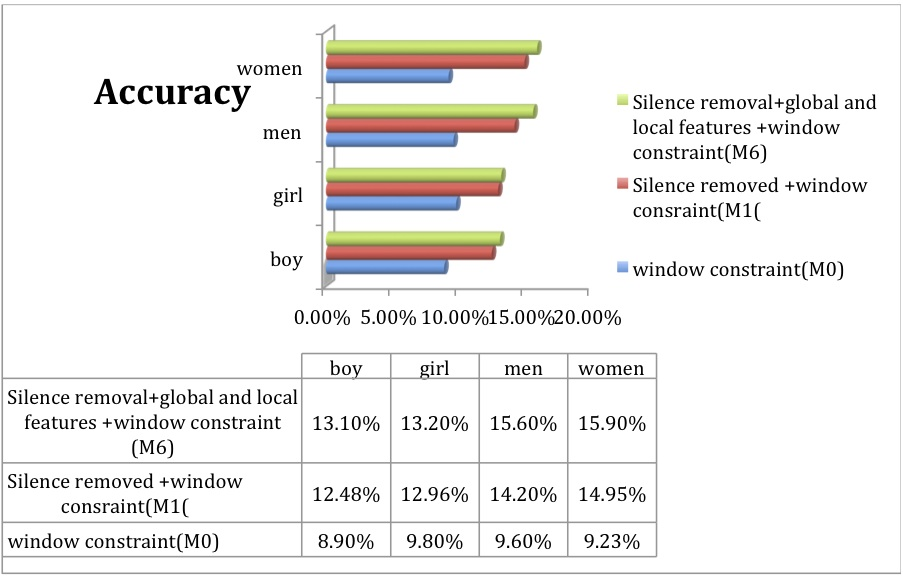
\includegraphics[scale=0.8]{425.jpg}
  \caption{}
  
\end{figure}
\begin{figure}[H]
  \centering
   
     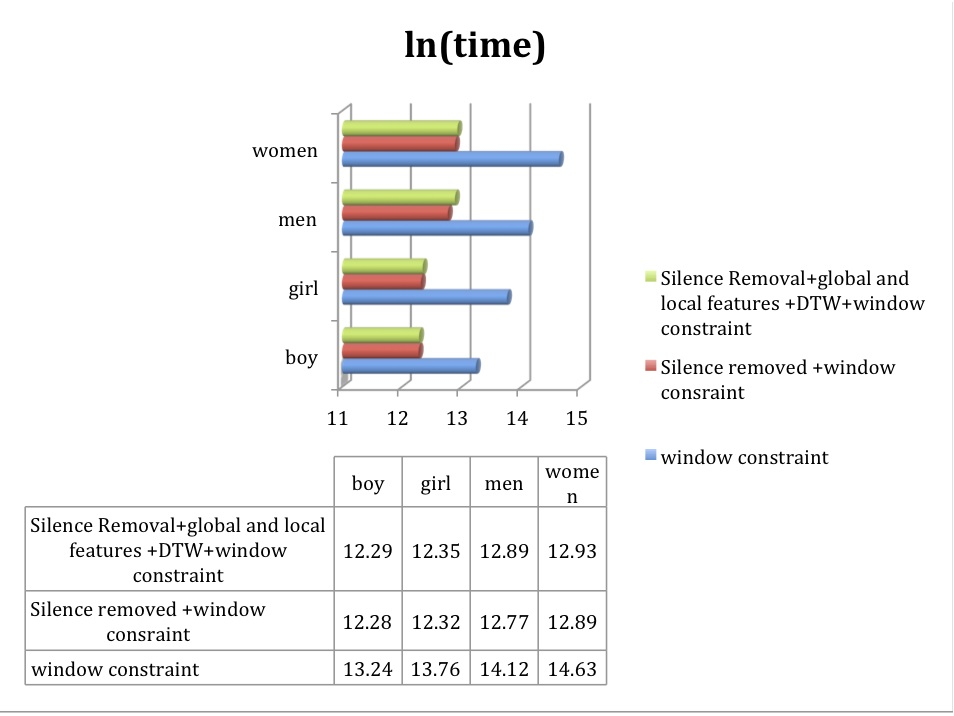
\includegraphics[scale=0.6]{426.jpg}
  \caption{}
  
\end{figure}
Observation:



 Surprisingly, by comparing these results with the previous experiments, it can now concluded that for the TIDIGITS dataset(2.1), removing redundant features i.e  removing regions of silence  is a greater contributing factor in improving the performance of a window constrained DTW than applying a feature extraction process that integrates meta data(4.2.1) or that captures information about local and global trends.   Using local and global features only leads to an average improvement of 0.8\%  over the model that performs only silence removal as a preprocessing step. 
 
 One obvious observation is the poor performance shown by all  3 models in terms of accuracy. From the analysis conducted so far, the reason for this poor performance can be narrowed down to  the use of the rigid window constraint imposed to minimise the time complexity.The computational cost incurred by the algorithm is higher than the version used for  the model of 4.1.1 One possible explanation is that the cost of applying the euclidean metric on vectors $> $cost of applying the euclidean metric on points. Since the euclidean metric is applied $mn$ times. The overall computational cost increases.



\item Experiment 2
Datasets: UCR datasets: InlineSkate and Cinc\_ECG\_Torso
\end{itemize}
The results are as follows:
\begin{figure}[H]
  \centering
   
     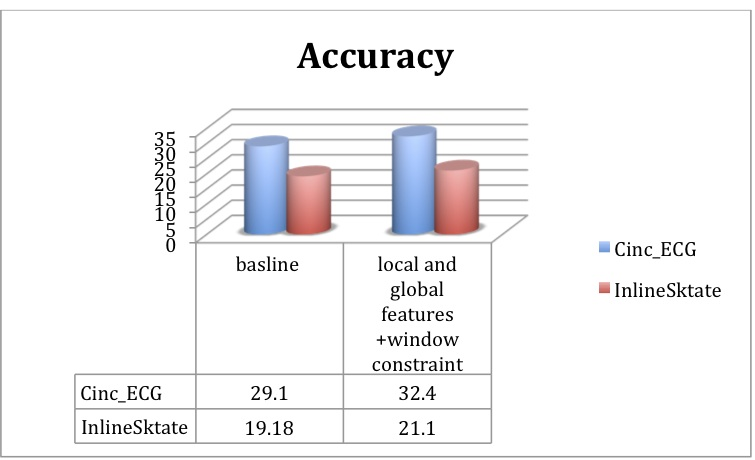
\includegraphics[scale=0.6]{427.jpg}
  \caption{Using features that reflect information of trends improves the accuracy of the algorithm}
  \end{figure}
\begin{figure}[H]
  \centering
   
     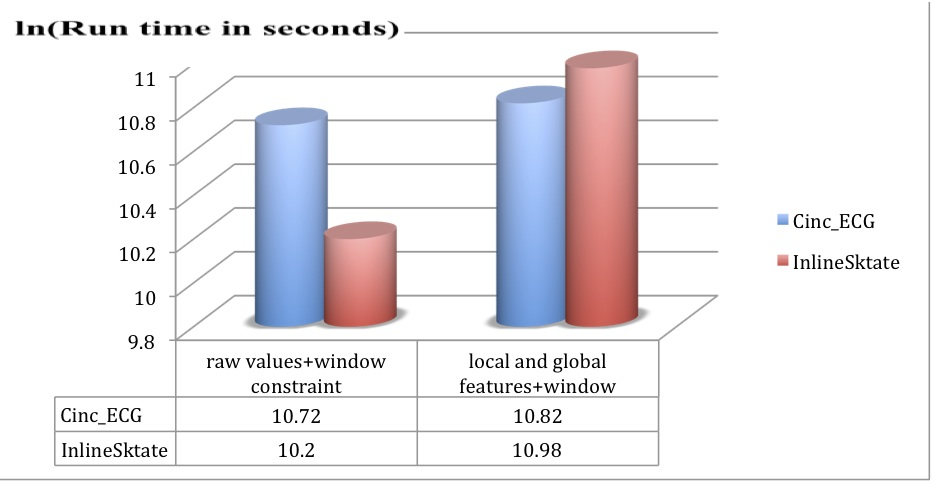
\includegraphics[scale=0.8]{428.jpg}
  \caption{The computation time incurred }
  \end{figure}
 
 \textbf{Observation} 
  \begin{itemize}
\item The differences between performances of  the two versions of DTW are consistent  with the observations made in the previous experiment. For the Cinc\_ECG\_Torso  time series data set, using global and local features improves the accuracy by 3.2\%  whereas  for the InlineSkate data set, the accuracy improves by 1.92\%.
Thus it is safe to conclude  that replacing each point in the time series sequence with a vector that reflect the relation of the point with the respect to the trends increase the number of the optimal warping paths that lie with in the regions bounded by the Sakoe-Chuba band constraint.The time complexity incurred by the algorithm under the new model is worse in comparison to the baseline model. Thus although  we achieve an improvement in accuracy, we are loosing  performance in speed. The accuracy of both the baseline and the current model is very low. This shows that a majority of the optimal warping between  sequences belonging to the same class lie outside the Sakoe-Chuba band.
  \end{itemize}

From the results of the experiments that has been conducted so far, it can be observed that the prominent factor responsible for the low accuracy of the DTW is the window constraint that keeps points(or vectors) of one sequence from getting too far from the other. Increasing the width of the Sakoe-Chuba band  will  although increase  the accuracy of the DTW (as seen in 4.2) but will definitely cause an reduction in speed. One of the primary goals of this project is to improve the performance of the DTW in handling sequences of high dimensionality(i.e log lengths). Thus \textbf{minimising} time complexity is as important as improving the accuracy. This provides the motivation to investigate alternative methods that can a better balance between the two conflicting goals of accuracy and speed. 

In the next section, I investigate a self-proposed method that is aimed  to help DTW tackle the two conflicting objectives  more effectively than using rigid window constraints. The new proposed methodology uses the data-driven feature extraction process that is discussed in the current section. The aim here to use the advantages presented by this domain independent feature extraction process [2] without being subject to the model's drawbacks.
% proposed methodology the DTW algorithm works on series of frames rather than series of vectors and employs a new kernel function(self-proposed) that is designed to measure the similarity of sub-sequences more accurately than standard euclidean metric by being \textbf{invariant} toward time-dilation and scale. (Details innext section).  

  
%To summarise, from the observation of the  results gathered from the  experiments it can be concluded that employing preprocessing steps that include the domain knowledge greatly improves the accuracy and time complexity of the DTW algorithm when high dimensional spaces and in some domain such the TIGITS corpus eliminates the necessity of impose global window constraints to achieve minimum computational cost.


 %n the previous chapter, I have investigated techniques on different pre-processing strategies that can improve the performance of the general  DTW algorithm  in working with high dimensional time series datasets. These techniques that I am investigated so far primarily focus on the improving the quality of the data rather than the algorithm itself. The results found from the experiments so far, have shown that understanding the intrinsic properties of the data and factoring in the  domain information can not only improve the performance of the  DTW but may even discard the need for a  the  global windowing constraint(as we have seen for the model that augments feature selection and MFCC feature extraction) to reduce the time and computational complexity.  The DTW algorithm is a memory based algorithm that employs a similarity metric to compare a sequence with all sequences in the training in an iterative manner.  Since the whole training set is used during the testing phase, the computational complexity makes the algorithm very attractive to use. The computational cost of a DTW algorithm is $(mn)$ where $m$ and $n$ denote the length of the two time series sequences currently being compared. Using longer sequences increases the size of the DTW cost matrix hence resulting into a greater number of computations. The domain-dependent pre-processing methodology doesnt guarantee the dropping of the  global window constraint that is used to reduce the search space when tackling high dimensional data. As we have seen from the experiments,when working with high-dimensional time-series data, the accuracy of the DTW algorithm using a window constraint suffers greatly even if it's equipped with domain dependent/independent features. Hence from a scientific point of view, it is of great interest to research methods to improve the DTW algorithm so it can constraint the time and computational complexity associated with high-dimensional data without degrading the accuracy by too much. In this chapter, I investigate an unsupervised methodology that:


 %Time series sequences are embedded with local and global trends. Unsupervised methods using DTW  focus on  exploiting the information of either these trends for pattern extraction and mining. From the  work conducted by Xie and Wiltgen on  the time series datasets[], it  has been shown that using DTW equipped with features that incorporate  information of \textbf{both}  local trends and global shapes in the clustering /classification process greatly improve the performance of DTW . Unlike the MFCC, the features constructed from local and global trends are domain independent and thus can be applied to any time of data.  However, when working high-dimensional time-series data, the accuracy of the DTW algorithm using a window constraint suffers greatly even if it's equipped with domain dependent/independent features. Hence from a scientific point of view, it is of great interest to research methods to improve the DTW algorithm so it can constraint the time and computational complexity associated with high-dimensional data without degrading the accuracy by too much. In this chapter, I investigate an unsupervised methodology that:

%\begin{itemize}
%\item incorporates  information about local and global trends  in the feature extraction process
%\item employs an adaptive DTW that tackles the issue of the large time and computational complexity by moving from working on  time series sequences to  sequences of segmented time-slices. To counter the tradeoff in the decrease  in accuracy, the algorithm is equipped with a kernel function(self-proposed) that is designed to measure the similarity of sub-sequences more accurately than standard euclidean metric by being invariant toward time-dilation and scale.   
%\end{itemize}
\section{Adapting  DTW}
The feature extraction methodology discussed above maps the time series sequence to a time series sequence of vectors whose length  is $\|X_n\|-2. $   ( where $\|X_n\| $ denotes the  length of the original time series sequence).  The DTW augmented with these features will still suffer from large time and computational complexity if the dimensionality of the data is high. In the MFCC feature extraction process, the time series sequence is first segmented into series of frames  of length 20ms i.e 200 points. Through appropriate functional mapping, each  frame is then mapped to a vector. Because the length of the resultant sequence of vectors is much smaller than the length of the original time series, the size of the  DTW cost matrix. This reduces the search space and thus decrease the time complexity of the DTW algorithm.

Using the MFCC feature extraction method as motivation, in the proposed model the sequence of 4d vectors extracted using the feature extraction process discussed in 5.1 are segmented using windows  of  size  50  which in the case of the speech data corresponds to width of 5 ms . The original time series is reduced to series of matrices where  the columns of the matrices consist of 4-d feature vectors corresponding to a particular time slice. The length of the series is now 50 times smaller than before. Now if we adapt the cost function of DTW to work on series of frames  rather than series of vectors as before we can achieve a large improvement in both accuracy and  computational cost  associated than imposing a \textbf{window} constraint. 

The problem now can be shifted to finding  an appropriate kernel that can be used to compute the similarity between matrices composed of feature vectors. Ideally, we want a metric that takes into account the variation of speed and time when comparing two similar subsequences. We will want to compare the global and local properties associated with a point in one subsequence with the global and local properties of points at  different regions in the second sub-sequence illustrated by figure 2.  Using a euclidean metric in this scenario is inappropriate. The euclidean metric  in this context is identical to  linear time warping where the  two subsequences will be matched based on a linear match of the two temporal dimensions.  In our context, we need a kernel that computes the similarity between two sub-sequences by warping the time axis.

The motivation behind the kernel  that I propose for aiding  DTW to tackle  high-dimensional sequences(i.e sequences with long lengths) comes from the polynomial kernel. \\
Let $x$ and $z$ be two dimensional vectors.
Consider the simple polynomial kernel of degree 2  :$k(x,z) = (x^{T}z)^2$ .  This kernel can expressed as :
\begin{eqnarray*}
k(x,z) &= &(x^{T}x')^2\\
&  =& (x_1z_1+x_2z_2)^2\\
&= & x_1^2z_1^2 + 2x_1z_1x_2z_2 + x_2^2z_2^2\\ 
&=& (x_1^2, �2x_1x_2, x_2^2)(z_1^2, �2z_1z_2, z_2^2)^{T}\\
&=& \phi(x)^{T}\phi(z)\\
\end{eqnarray*}\\
The 2nd order polynomial kernel is equivalent to a corresponding feature mapping $\phi(x)$  that  maps a two dimensional vector to $x_1^2, �2x_1x_2, x_2^2)$ where each attribute is monomial of order 2 .  Generalising this notion to order M then $k(x,z) = (x^{T}z)^M$ contains all monomials of order M.  Now, if we imagine x and z to be two images, then the polynomial kernel represents a particular weighted sum of all possible products of M pixels in the first image with M pixels in the second image.\\
Using this as motivation I propose the following kernel:.
\[ k(x,z) = <\sum_{i=1}^{n}x_i, \sum_{j=1}^{n}z_j>\]
where $n$ denotes the length of the window and $x_i$  and $z_j$ represents the 4-dimensional features indexed by the points in two sub-sequences.\\
To motivate the reasoning behind the construction of this particular kernel lets consider the following signals:
\begin{figure}[H]
  \centering
   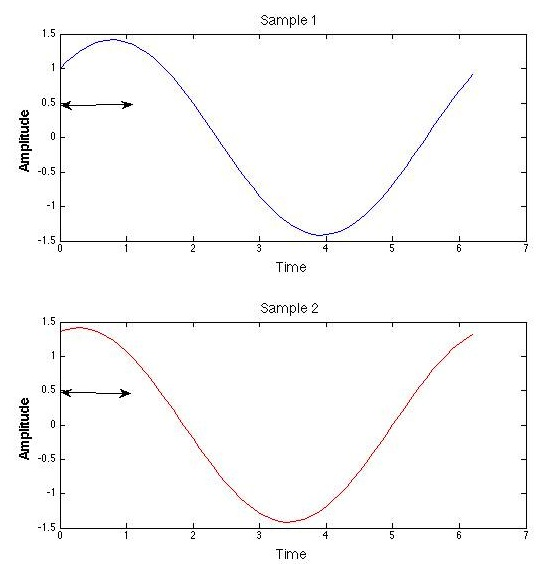
\includegraphics[scale=0.4]{Example1.jpg}
  \caption{Two signals separated by translation}
 \end{figure}
The signal denoted by the `red' color is a `slower' version of the signal denoted by the `blue' color . In the above example, if we are comparing the similarity  between the  time slices spanned by the arrows, an ideal kernel must be invariant to  the time offsets of the signals and thus should consider all possible pairings between the vectors in the subsequences. Intuitively speaking, the kernel must behave like a DTW algorithm.\\
\begin{figure}[H]
  \centering
   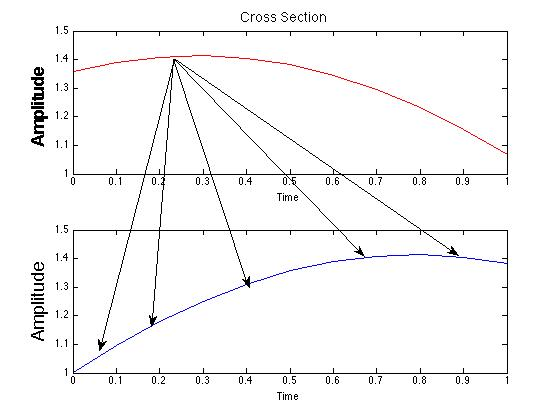
\includegraphics[scale=0.6]{Cross-section.jpg}
  \caption{Two identical subsequences varying in time }
  \end{figure}
 For time slices of width $n$, the kernel  metric  can be expanded and   expressed as :
\begin{eqnarray*}
k(x,z) &= &<\sum_{i=1}^{n}x_i, \sum_{j=1}^{n}z_i>\\
&  =& <(x_1+x_2+x_3+..),(z_1+z_2+z_3+..)>\\
&= & <x_1,z_1>+<x_1,z_2>+<x_1,z_2>...+<x_2,z_1>+<x_2,z_2> +<x_2,z_3>+......\\ 
\end{eqnarray*}
From above expression, we can see  that the proposed kernel corresponds to a sum of all possible dot products of pairs belonging to the set
$\{(x_iz_i) | x_i\in \mbox{seq1}, z_i \in \mbox{seq2}\}$. Similar to the polynomial kernel, the proposed kernel  allows us to match all possible pairs of vectors belonging to the two sub-sequences  given by the matrices.
It is easy to check that this proposed kernel is in fact a valid kernel:
\begin{itemize} \itemsep-2pt
\item K(x,z)= K(z,x) $\Rightarrow $the function is symmetric.
\item The kernel satisfies Mercer's theorem : K(x,z) =$\phi(x)^T\phi(x)$
where  the feature mapping corresponds to  a finite summation of vectors $\phi(y) = \sum_{i=1}^{n}y_i$. 
\end{itemize}

Augmenting the kernel to the DTW algorithm allows DTW to work on high-dimensional time sequences without using a window constraint. However the accuracy and computational cost of the DTW is now dependent on the size of the time slices used to segment the original sequences in the first place.
%\begin{itemize} \itemsep-2pt
%\item The accuracy of DTW increases as the width of the windows decrease. Using subsequence allows the similarity measure to be dominated by the dot products of points whose local and global features are most alike. However using smaller windows achieve lesser dimensionality reduction. Thus the time and computational complexity suffers.
%\end{itemize}
To use this kernel as an  appropriate cost function in the DTW algorithm, we need a functional mapping that:
\begin{enumerate} \itemsep-2pt
\item  constraints the codomain to be in the range from 0 to $\infty$.
\item    ensures larger values given by the function signify great degree of dissimilarity and smaller values  signify a high degree of similitude.
\end{enumerate}
An ideal cost function that make use of dot products is the \emph{arc-cosine}. Hence I embedded the kernel function in the cosine distance: 
\[ \theta = \frac{ <X,Z>}{|X||Z|} \]
where $X = \sum_{i=1}^{n}x_i$ and $Z =\sum_{j=1}^{n}z_i$

A formal outline of the algorithm is as follows:

 \begin{algorithm}
\begin{algorithmic}[1]
\Procedure{Value-based}{$seq1,seq2$}\Comment{two sequences of feature vectors}
\State  seq\_1$\leftarrow$segment(seq1,n)\Comment{ Segment the sequences using a window of size n}
 \State seq\_2$\leftarrow$segment(seq2,n)
 \For{i=1: to length(seq\_1) } \Comment{Initialise the DTW cost matrix}
 \State DTW(i,0) = $\infty$
 \EndFor
 
 \For{i=1 to length(seq\_2)}
 \State DTW(0,i) = $\infty$
 \EndFor
  \For{i=2 to length(seq\_1)}  
 \For{j=max(2, i-w) to min(length(seq\_2), i+w)} 
 
  \State DTW(i,j) = $\theta = \frac{ <X,Z>}{|X||Z|} $+ min\{ DTW(i-1,j)+DTW(i,j-1)+DTW(i-1,j-1)\}
 \EndFor \Comment { $X = \sum_{i=1}^{n}x_i$ and $Z =\sum_{j=1}^{n}z_i$}

 
 \EndFor
\State \textbf{return}  result = $\frac{\mbox{DTW(n,m)}}{nm}$ \Comment{n=length(seq1), m=length(seq2)}

\EndProcedure
\end{algorithmic}
\caption{Adapted DTW}
\end{algorithm}
 


\subsection{Testing the methodology}
The changes that I have introduced  in the previous section  to the `Dynamic Time Warping' algorithm is aimed to improve the algorithm's performance in handling long time series sequences. In this section, I investigate  the performance of my proposed  methodology against  the versions of the DTW algorithm that employ the Sakoe-Chuba band constraint (discussed in 4.1.1). To reduce the time complexity to a minimum, the window constraint that I have used so far is the most rigid constraint that can be imposed on the DTW algorithm without forcing the algorithm to behave like the euclidean metric. In order to measure the difference in performance between using my proposed method  and  employing  the window constraint, I have conducted the following  experiments:


\textbf{Experiment 1}

\textbf{Data set used} : The TIDIGITS test and training data.

\textbf{Model Used} : The model discussed in 5.2. The model framework consists of a two stage preprocessing step that involves feature selection process consisting of `silence' removal  followed the domain  independent feature extraction discussed in the previous section.

\textbf{Variables being compared}: employing window constraints vs the  new proposed changes

RESULTS: the results are as follows:
 \begin{figure}[h!]
  \centering
      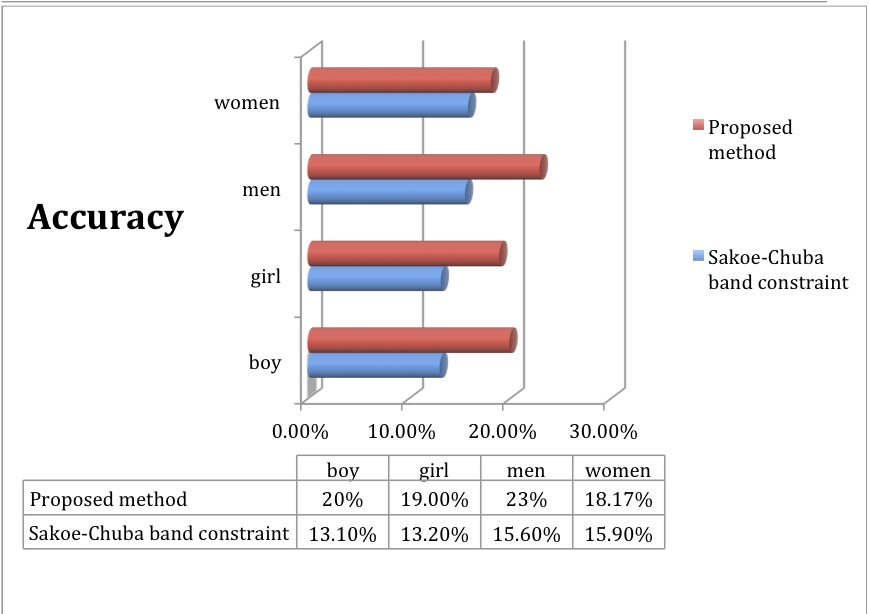
\includegraphics[scale=0.9]{521.jpg}
  \caption{Accuracy}
  \end{figure}

\begin{figure}[H]
  \centering
     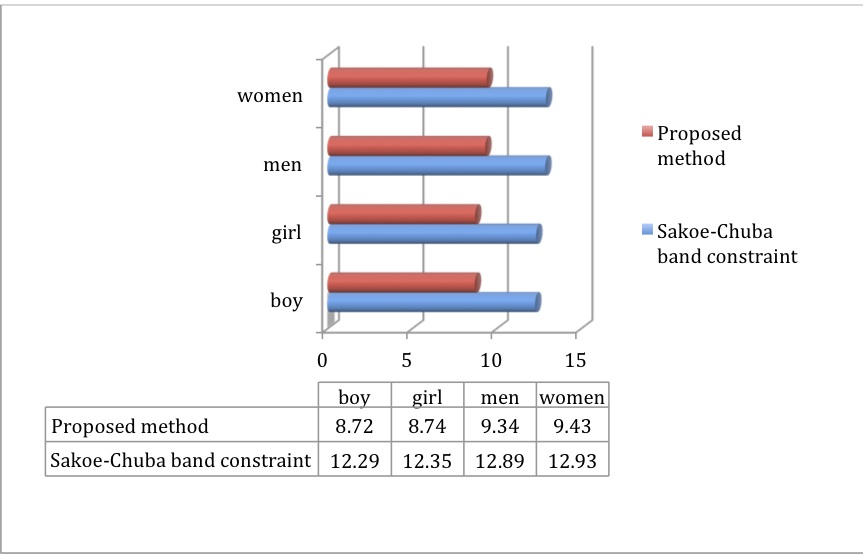
\includegraphics[scale=0.9]{522.jpg}
  \caption{Time complexity in log(time)}
  \end{figure}

There are quite number of interesting observations that can made from the graphs and the tables given by figures 5.7 and 5.8. 

\begin{itemize}
\item The proposed changes  to DTW allow the algorithm to achieve better accuracy on test samples across all categories than employing the  rigid Sakoe-Chuba band constraint  of  $w = max(\lceil{0.1*max(n.m)}\rceil, abs(n-m))$.  The most interesting result is that the new algorithm incurs a lower computational cost than before.Thus introducing these changes have improved both the accuracy and time complexity of the algorithm.  From the results noted in the tables, it can been seen that the accuracy of DTW  has increased by 6.54\% on average and the average log(time) has decreased by 3.1. The reduction of the time complexity is mainly due to the partitioning of the sequence into  time slices of width  5 ms. The reduction in  the length of the sequences by an order of 50 results in the shrinkage of the search space of DTW thus causing the algorithm to improves its speed. As we have seen so far, increasing the speed of DTW negatively impact the accuracy, in this scenario, the new methodology actually provides an exception. The use of the kernel function improves the accuracy of the DTW   which implies that matching frames using the new cost function is a better alternative than employing the euclidean distance between points/vectors confined by the window constraint.

In the previous chapter, we have seen that  for the TIDIGITS data set,  constructing a preprocessing methodology that involves `silence' removal followed by MFCC feature extraction allows DTW to minimise its time complexity and at the same achieve high accuracy without the use of the  global window constraint. However for situations where the need for a global window constraint is deemed necessary, it will be interesting to investigate whether the new changes do in fact provide a better alternative to using rigid window constraint for  very long sequences. To check that the new changes allow DTW to perform equally well using domain dependent features,   I have repeated the same experiment again but this time, as  a preprocessing step  I have  just used  the MFCC feature extraction 

A summary of the results are as follows:
\end{itemize}
\textbf{Experiment 2}

\textbf{Data set used} : The TIDIGITS test and training data.

\textbf{Model} : The model framework consists of single preprocessing step that involves the extraction  of MFCC features

\textbf{Variables being compared}: employing window constraints vs the  new proposed changes
\begin{figure}[h!]
  \centering
      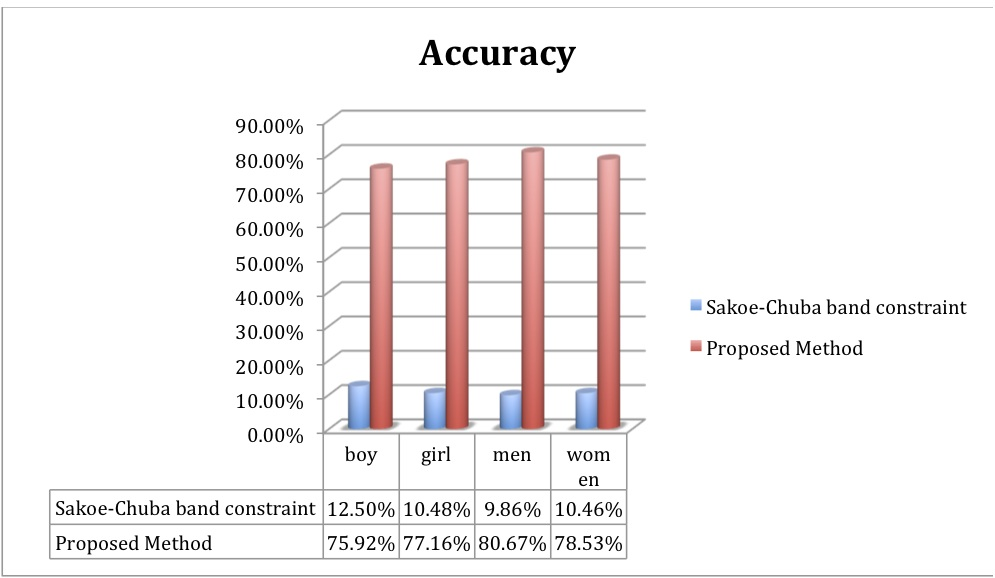
\includegraphics[scale=0.9]{523.jpg}
  \caption{Accuracy}
  \end{figure}

\begin{figure}[H]
  \centering
     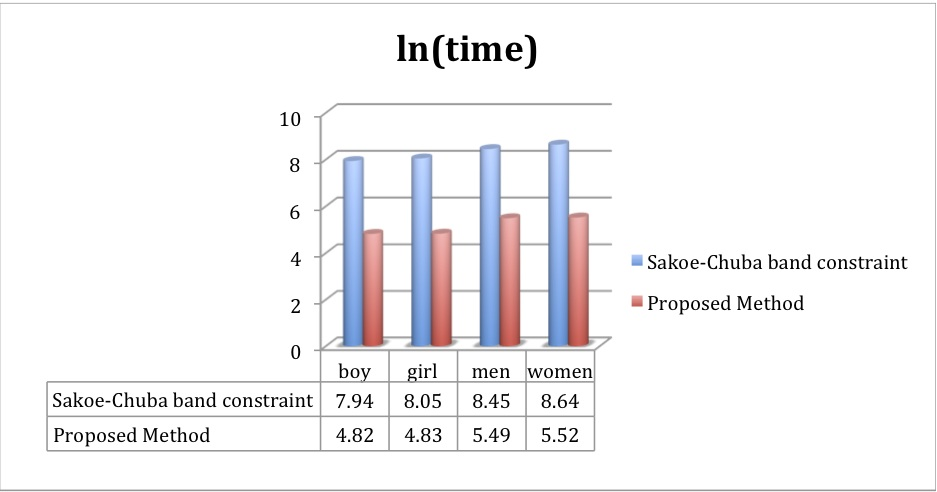
\includegraphics[scale=0.9]{524.jpg}
  \caption{Time complexity in log(time)}
  \end{figure}

\textbf{Observation}

From the above results, it can be observed that the new changes does provide an a \textbf{ better} alternative approach  to using a very rigid constraint for scenarios where the time complexity is of high priority and the use of window constraints can not be avoided.  For this data set, using the new approach improves the accuracy of the DTW by over 60\% and the log( time)  is reduced by order. This shows that that not only the time complexity is exponentially reduced but the accuracy has also been boosted.  However, since the tests so far has been conducted on the TIDIGITS test set, it is possible that this new approach is only tailored for this particular data set. Thus to confirm  that the performance of the new algorithm  is not tailored for this particular time-series data set, I have the test the performance of the DTW augmented with  the new changes on the UCR data sets: InlineSkate and CINC\_ECG\_TORSO.

\textbf{Experiment 3}

\textbf{Data sets used} : InlineSkate and CINC\_ECG\_TORSO

\textbf{Setup} : One of the main goals of this analysis is to construct a methodology that can achieve  good performance in both speed and accuracy across multiple domains. The model framework that I am using for this experiment involves the use of  the feature extraction process discussed in 5.1 and [2].  From the experiments conducted on the UCR datasets, Xie and Witgen[2] have shown  at the cost of higher computational complexity m the accuracy of the DTW algorithm does improve by a significant amount when the algorithm substitutes each raw value with a 4-d vector  that reflects information about local and global  trends. However, from the analysis I conducted in 5.1, it was observed that under the window constraint, the use of these features made little contribution in improving the performance of the algorithm. If  replacing the window constraint with the new changes does improve the performance of the DTW algorithm then we will have a model where the use of global and local features  does allow the algorithm to achieve greater performance even when the decreasing the time complexity is a major priority. 

In the  proposed approach,  the width of the time slices has been kept fixed at a default value of 50 so far. In this experiment, I also investigate the influence of this parameter on the performance of the DTW. Decreasing its value reduces  the size of the time slices which in  principal should increase both accuracy and time-complexity .
The core kernel used by the new algorithm is based on the function: 
\[ k(x,z) = <\sum_{i=1}^{n}x_i, \sum_{j=1}^{n}z_j>\]
k(x,z) represents the sum of all possible dot-products. Using smaller subsequences allow the similarity measure to be dominated by the dot products of points whose local and global features are most alike. However,  this suffers from the drawback of achieving lesser dimensionality reduction. Thus the time and computational complexity suffers.

\textbf{RESULTS}

\begin{figure}[H]
  \centering
      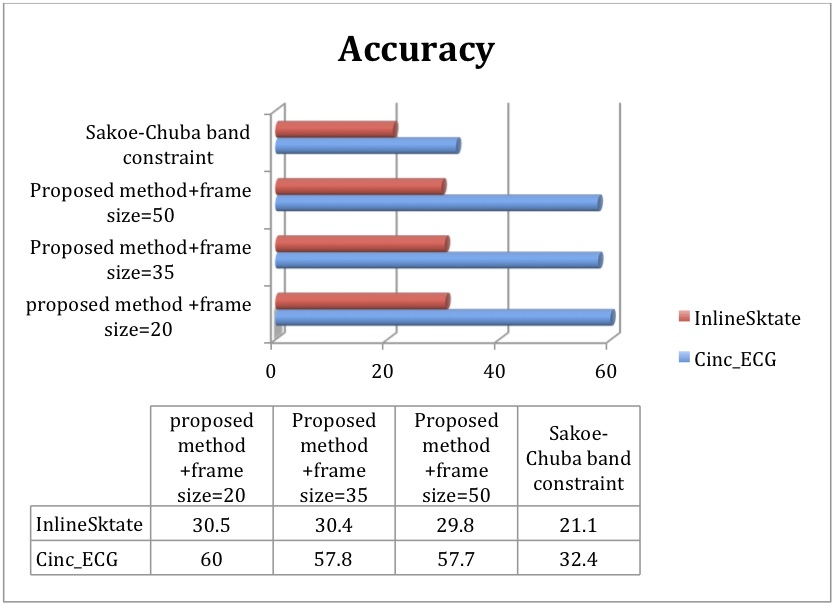
\includegraphics[scale=0.9]{525.jpg}
  \caption{Accuracy}
  \end{figure}

\begin{figure}[H]
  \centering
      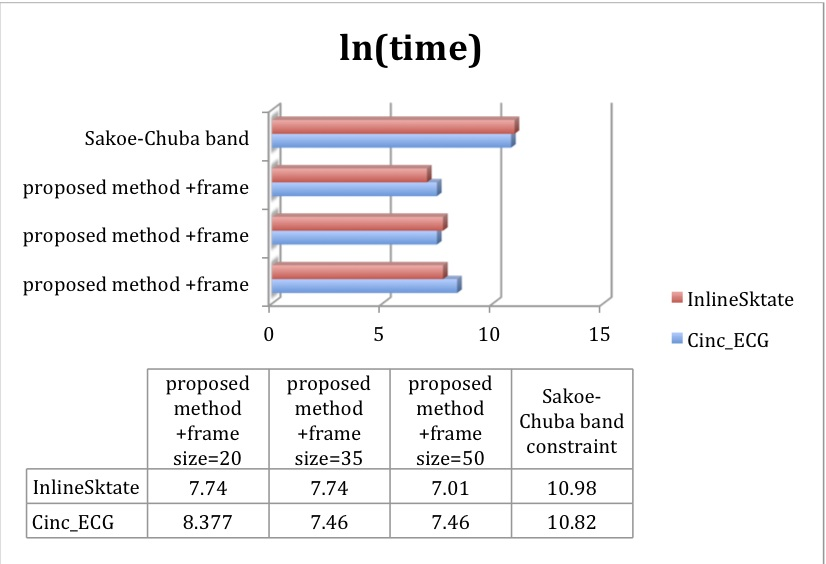
\includegraphics[scale=0.9]{526.jpg}
  \caption{Accuracy}
  \end{figure}

\textbf{Observation}

\begin{itemize}
\item The proposed changes does provide  a \textbf{ better} alternative approach  to using rigid constraints  for problem domains where the time complexity is of high priority and the use of window constraints can not be avoided. The accuracy of the DTW algorithm under the new methodology is significantly higher then employing a window constrained DTW on sequences of extracted local and global features.  In my analysis in 5.1, I have already shown that the latter model achieves  better accuracy than the baseline model. Thus the new methodology improves the performance of the DTW in both speed and time and also can be \textbf{applied} to time series sequences belonging to different domains. Hence, combining this approach with the feature extraction method discussed in [2]  results in the construction of a model that can applied for \textbf{different types} of time series data sets. 
 \item Decreasing the size of the time slices only leads to a minimal increase in accuracy. Thus using the default value of 50  seems to be safe option as the algorithm better accuracy and speed than using the rigid Sakoe-Chuba band constraint .
\end{itemize}
   
%% ... etc ...

%%%%%%%%
%% Any appendices should go here. The appendix files should look just like the
%% chapter files.
%\appendix

\bibliographystyle{ieeetr}
 \bibliography{../../../../../Documents/mendeley/library.bib}

%% ... etc...

%% Choose your favourite bibliography style here.
%% If you want the bibliography single-spaced (which is allowed), uncomment
%% the next line.
% \singlespace

%% Specify the bibliography file. Default is thesis.bib.

% 100 is a random guess of the total number of 
%references
%% ... that's all, folks!
\end{document}
